\section{RL-BRT Model}
\label{sec:model}

\begin{figure}[htbp]
	\hspace{0ex}
	\vspace{0ex}
	\centering
	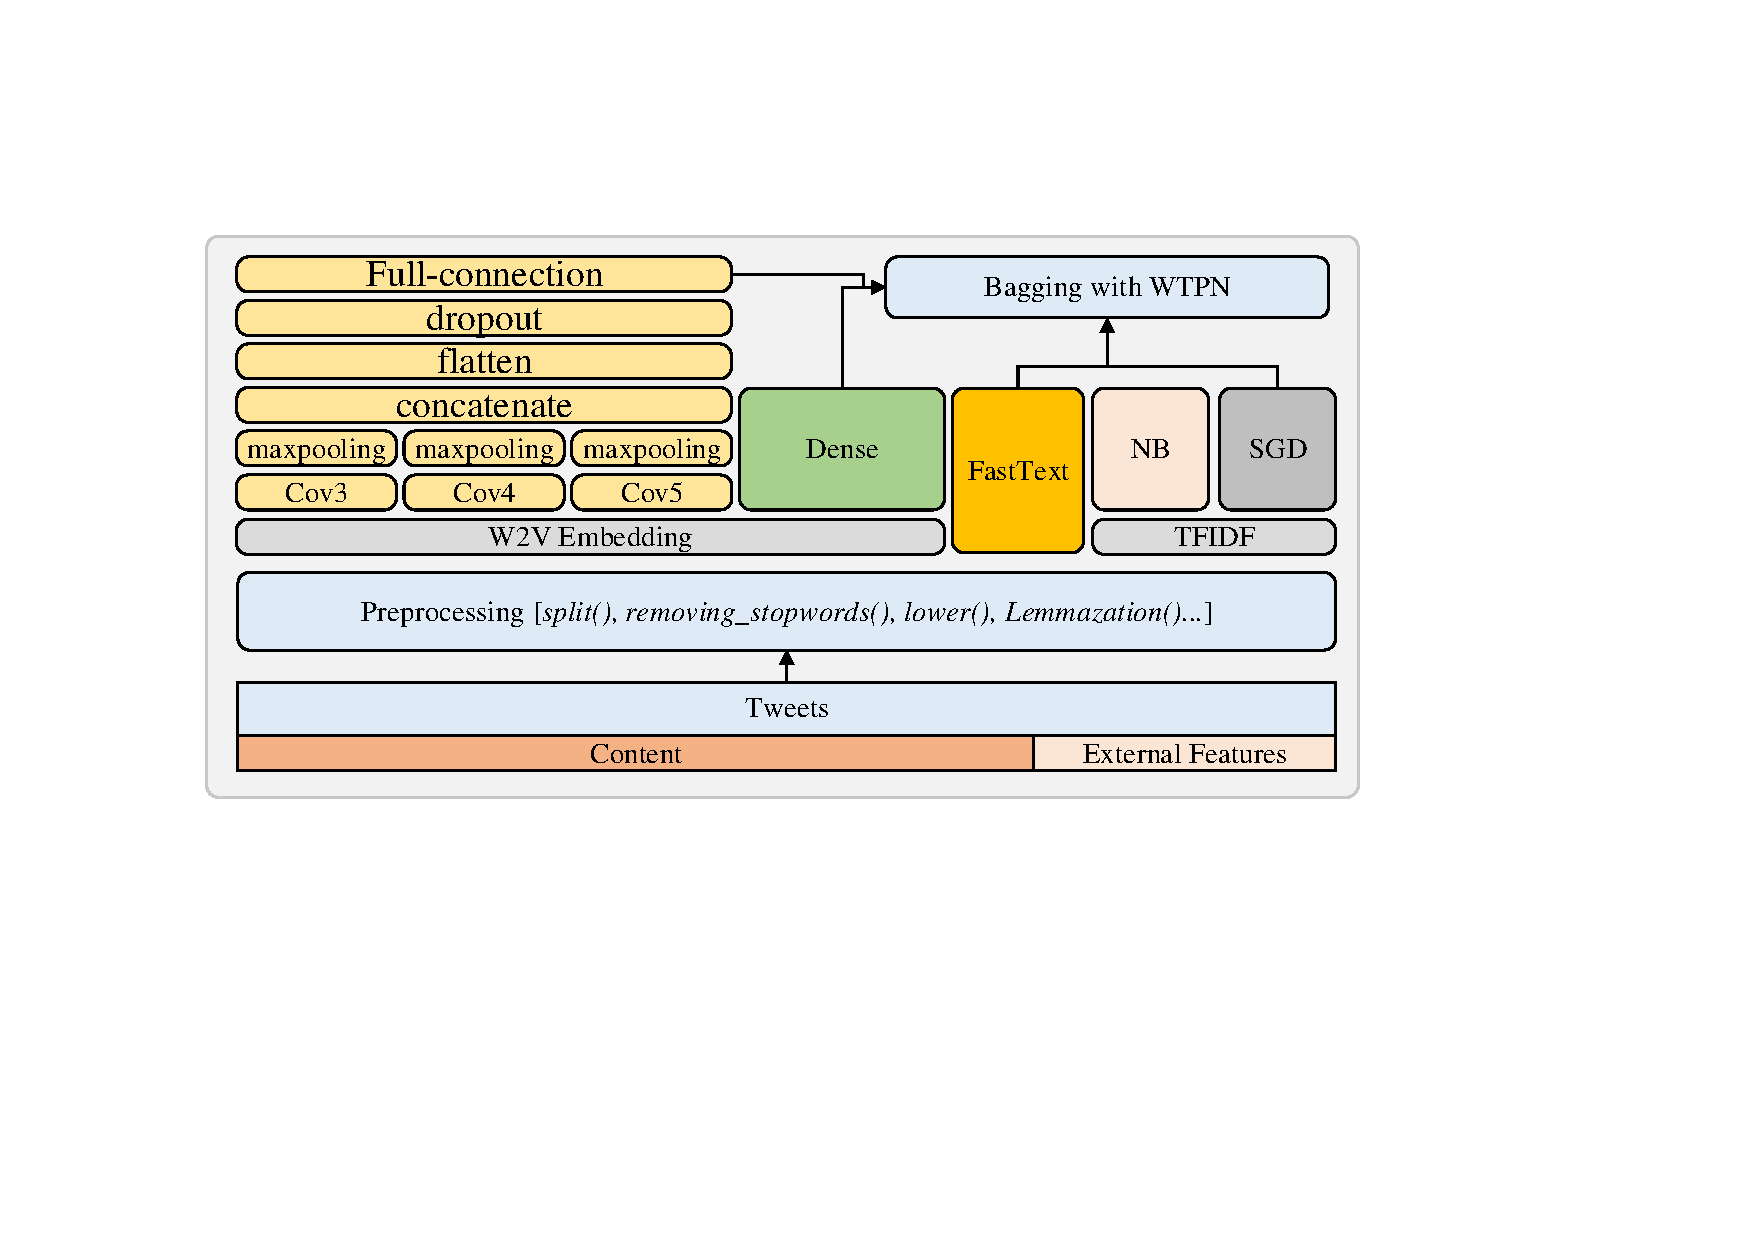
\includegraphics[width = \textwidth]{fig/structure}
	\caption{Architecture of RL-BRT}
	\label{fig:architecture}
\end{figure}

Bagging (Bootstrap aggregating) model \cite{DBLP:journals/ml/Breiman96b} aggregates different basic models as its components. With a proper bagging strategy, the performance is usually better than that of the basic models. Bagging model reduces variance and improves the
stability of estimated density. Besides, the multiple components balance each other to reduce overfitting. Also, the most suitable classifier for different types of features is changing, and therefore multiple components are more likely to contain the proper classifier. Moreover, the importance of components changes according to the sample. Therefore, we propose a reinforcement learning based weight-tuning policy network (WTPN) to generate a suitable weight to balance the importance of components for each sample. 

\subsection{Architecture}
\label{sec:architecture}
The architecture of RL-BRT is shown in Fig. \ref{fig:architecture} . The input of  RL-BRT consists of two types of features, which include content features and social features. Then, all features are embedded and sent to basic components.  Some components such as TextCNN and Dense use word-to-vector embeddings and the other components use particular embedding methods. Next, each trained component makes its prediction separately. Finally, we add the predicted results of all components and generate a final prediction by a reinforcement learning based bagging algorithm.

\subsection{Preprocessing and Embedding}
\label{sec:process_embedding}
The textual content is one of the most important features in rumor tracking task. The length of the textual content is short, which is restricted within 140 words. Usually, the spelling in tweets is causal with symbols mixed in it. Consequently, we clean the content before inputting them into the model. The preprocessing in NLP is roughly immobilized, we only make some minor adjustments. In this work, we adopt splitting on tweets, and then remove the punctuation and special characters. Next, we turn all characters into lowercase. Finally, we adopt lemmatization on all words.

We find that the embedding strategies have a significant impact on the performance of RL-BRT. Therefore, we try different embedding strategies to find the most proper one. There are three commonly used embedding strategies: pre-trained embedding, self-trained embedding, and random embedding. Pre-trained embedding is trained on large-scale corpus, and the most representative ones are GloVe \cite{DBLP:conf/emnlp/PenningtonSM14} and Google News embedding \cite{googlenews}. The self-train embedding is to train embedding on the current dataset. And the random embedding is to assign each word to a unique embedding randomly. In this work, we try all three embedding strategies and the detailed performance is introduced in Section \ref{sec:experiment}. By comparing them, we finally choose random embedding as the embedding strategy in RL-BRT.

\begin{algorithm}[tbp]
	\caption{Bagging Algorithm}
	\label{algorithm:RL-BRT}
	\LinesNumbered % show line numbers
	\KwIn{$K_y = \left\{y_F', y_T', y_B', y_N', y_S' \right\}$: outputs of all components;
		$x \in R^{l \times d}$: a processed sample;
		$WTPN$: weight-tuning policy network}
	\KwOut{$R$: predicted result of RL-BRT;}
	\textbf{Initialize:} Outputs of RL-BRT: $y' = [0]*m$, $R = 0$ \;
	$W_y =  WTPN(x, K_y)$ \;
	\For{$i$ in $\{F,T,B,N,S\}$}{
		$y'+= w_i \cdot y_i'$;
	}
	
	$R = argmax(y')$
\end{algorithm}

\subsection{Procedure of RL-BRT}
As shown in Fig.~\ref{fig:architecture}, after embedding, we send \textbf{content features} into TextCNN, SGD, and FastText. These three components are trained respectively until getting convergence. When predicting, each component outputs an m-dimensional vector $y'$ after the softmax layer. Each component in $y'$ indicates the probability of the content belongs to this category. Despite some content features, the tweets contain plenty of \textbf{social features}. As introduced in Section \ref{sec:problem}, the tweet's branch or thread is unknown in advance. Consequently, we omit some features that contain external information about the branch or thread. Finally, we choose ``screen name", ``reply to screen name", and ``hashtag" as the social features in RL-BRT. We treat the social features as words and add them to the tweets. Then we send the tweets with social features into NB and SGD. 

With all components in RL-BRT trained, we aggregate them and make a final prediction on the rumor tracking task. Generally, frequently used bagging methods include \textbf{joint training} and \textbf{respective training}. Joint training means all models have one shared loss function, and all parameters are updated together. When predicting, the bagging model directly outputs the final prediction. Respective training means we train each component respectively. When predicting, each component makes its prediction result. In RL-BRT, we choose the respective training. 

As all components are trained, results are aggregated by a bagging algorithm. The bagging details of RL-BRT are shown in Algorithm~\ref{algorithm:RL-BRT}. We denote the predicted result of RL-BRT as $R$. The inputs of Algorithm~\ref{algorithm:RL-BRT} are a sample $x$ and its predicted results of all components, which are denoted as $K_y = \left\{y_F', y_T', y_B', y_N', y_S' \right\}$. Each element in $K_y$ is an m-dimensional vector. Then, $x$ and $K_y$ is sent to WTPN and the output is a set of weights denoted as $W_y$ (Line 2). Each element $y_i'$ in $K_y$ is assigned with a weight in $W_y$. Next, we sum the predicted results in $K_y$ with weights (Line 4). Finally, the category with the maximum possibility is the predicted result of RL-BRT (Line 6). 

\begin{figure}[tbp]
	\hspace{0ex}
	\vspace{0ex}
	\centering
	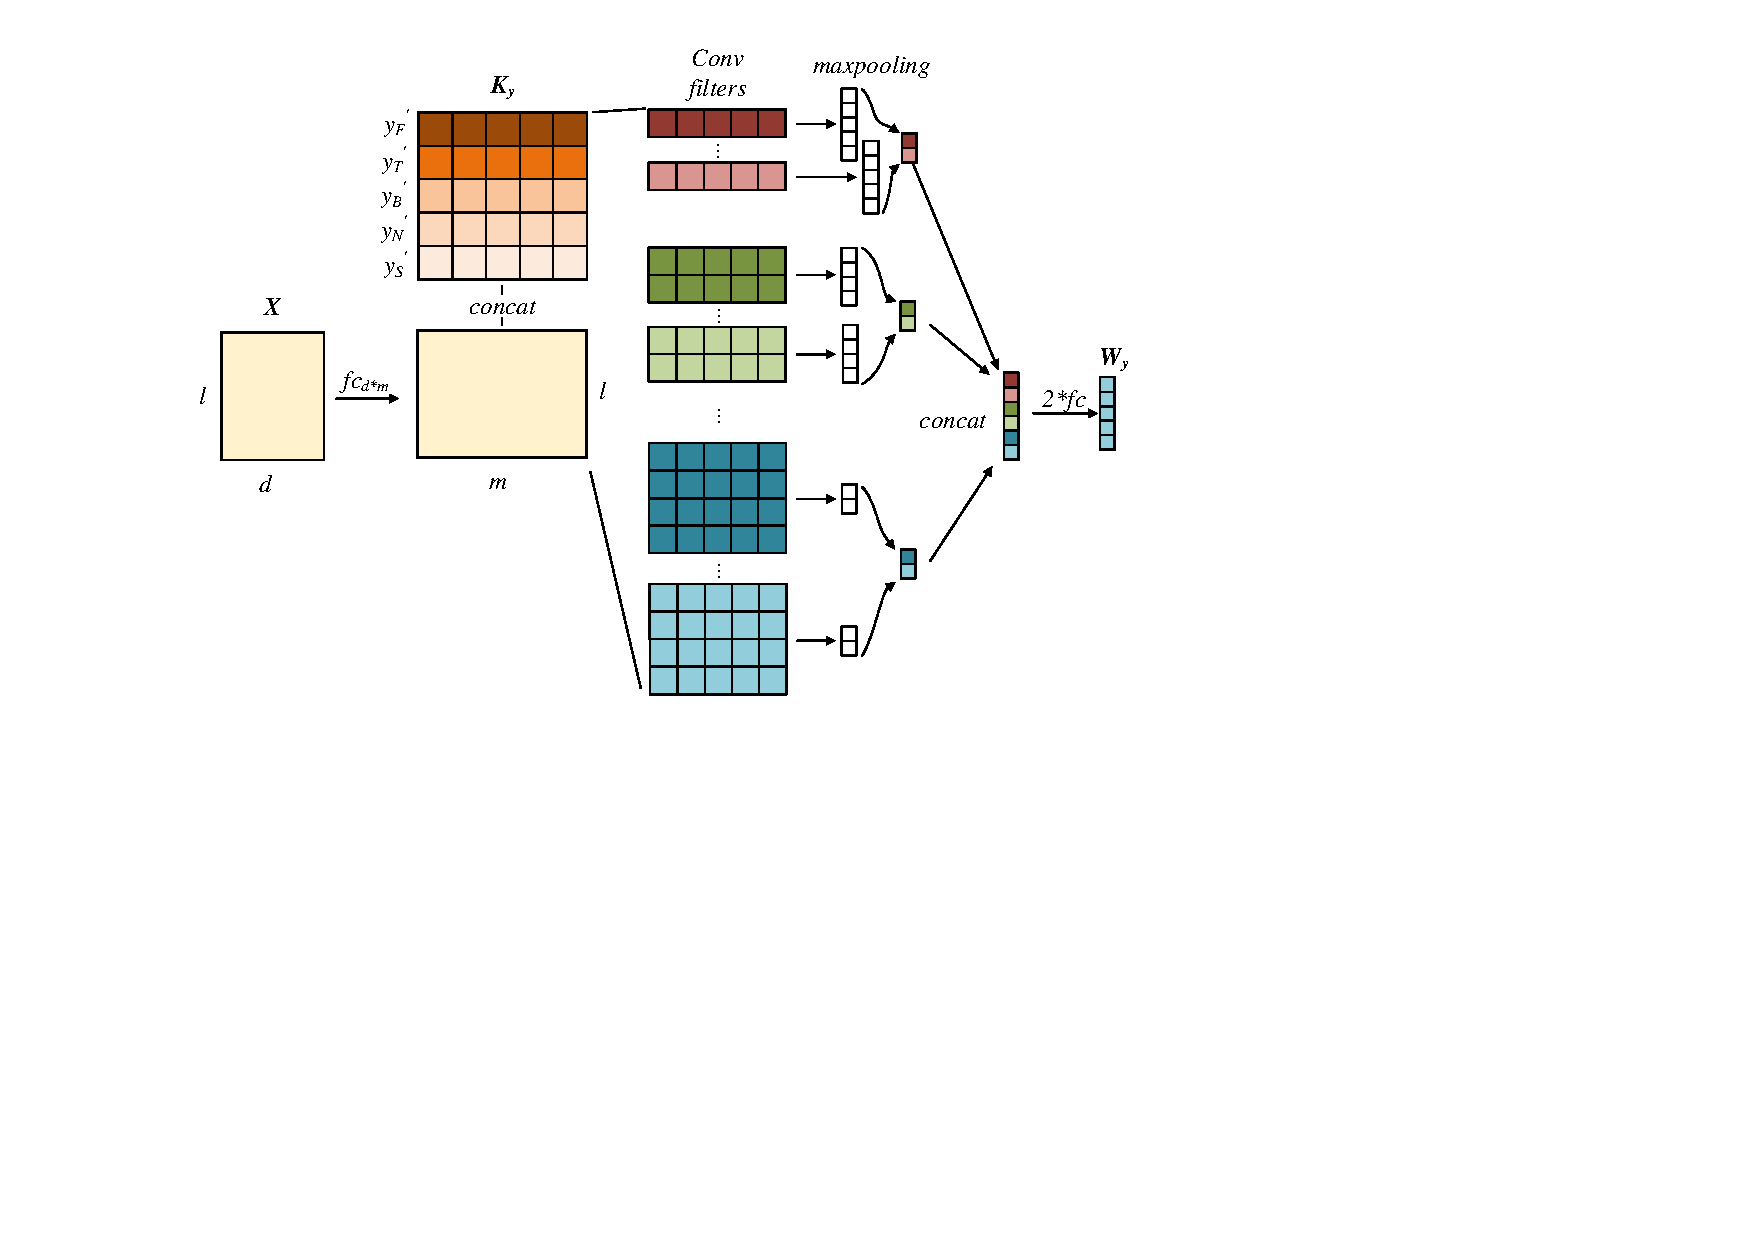
\includegraphics[width = \textwidth]{fig/WTPN}
	\caption{Structure of WTPN}
	\label{fig:WTPN}
\end{figure}

\subsection{Weight-Tuning Policy Network}
We propose WTPN to generate a suitable weight for each sample. WTPN is based on a reinforcement learning structure with a triple-tuple $<S, A, R>$, where $S = \{ s \}$ is a set of states. $A = \{ a \}$ is a set of actions. $R(s, a)$ is the reward function.
\begin{itemize}
	\item \textbf{State} $s$: $s = ( x, K_y )$ denotes a state of WTPN, where $x$ is a sample and $K_y$ is the set of classification results of $x$ generated by different classifiers.
	
	\item \textbf{Action} $a$: $a = W_y$ denotes a set of weights corresponding to elements in $K_y$.
	
	\item \textbf{Reward} $R$: $R(s, a) \to r \in R^{S * A}$ is a reward function that measures the profit of the current state-action tuple $(s, a)$.
\end{itemize}

For a batch of samples $X_b$, the accumulated reward is defined as:
\begin{equation}
R(s_1, a_1, ..., s_{|X_b|},a_{|X_b|}) = \frac{1}{|X_b|}\sum_{t = 1}^{t = |X_b|} r_t,
\end{equation}
where $ \frac{1}{|X_b|}$ is a normalization item. For a sample, $R(s,a) = r$ is the negative softmax cross-entropy loss between the predicted result (Line 6 in Algorithm \ref{algorithm:RL-BRT}) and ground-truth label.
For each batch, the parameter $\theta$ of policy function is updated by the following equation: 

\begin{align}
\theta &\leftarrow \theta + \lambda \nabla_\theta J_b(\mu_\theta),\\
J_b(\mu_\theta) &= \mathbb{E} [R(s_1, a_1, ..., s_{|X_b|},a_{|X_b|}) ],
\end{align}
where $\lambda$ is learning rate. $J_b(\mu_\theta)$ is the expected return.

The goal of WTPN is to approximate a policy function $\mu_\theta :S \to A$ that maximizes the accumulated reward.  Inspired by \cite{DBLP:conf/aaai/KimJSR16}, we propose a CNN based WTPN structure. As shown in Fig.~\ref{fig:WTPN}, the inputs of WTPN are $x$ and $K_y$ and the output is $W_y$. $x$ is sent to an FC (full-connect) layer and concatenated with $K_y$. We adopt multiple filters on the concatenated vector. The sizes of multiple filters are different, including  $[2*m]$, $[3*m]$, $[4*m]$, and $[5*m]$. The convolutional padding strategy is the same. By convolution and max-pooling, WTPN concatenates the captured features. Finally, with 2 FC layers, WTPN outputs $W_y$. 